\documentclass[12pt]{article}
\usepackage[a4paper, total={6.6in, 9in}]{geometry}

%\setlength{\parskip}{3pt}

\usepackage{amsmath}
\usepackage{amssymb}
\usepackage{bm}
\usepackage{graphicx}
\usepackage{siunitx}
\usepackage{authblk}
\usepackage{url}
\usepackage{appendix}

\bibliographystyle{ieeetr}

\begin{document}

\title{Can liquid crystal phases be identified via machine learning?}
\author{Joshua Heaton 10133722}
\affil{School of Physics and Astronomy, The University of Manchester}
\affil{MPhys project report}
\date{\today}

\maketitle

\begin{abstract}
hi
\end{abstract}

\pagenumbering{gobble}
\newpage
\pagenumbering{arabic}

%=========================================================================================
\section{Introduction}
Machine learning methods have seen widespread utilisation across all scientific disciplines, in situations where conventional algorithms are too cumbersome to implement for specific data-based and modelling tasks \cite{Carleo19}. Deep learning, loosely defined as machine learning with large datasets, parallel computation and scalable algorithms with many layers \cite{Goodfellow16}, has and continues to increase the range and complexity of possible applications of machine learning in the sciences \cite{Carleo19}. Any task applying deep learning to data with a grid-like form, such as images, likely involves the usage of convolutional neural network (CNN) algorithms \cite{Goodfellow16}. CNNs were conceived in 1989 by Yann LeCun \textit{et al.} and successfully applied to recognition of handwritten characters \cite{LeCun89}. However, their astounding performance in the field of computer vision would not be fully realised until after breakthroughs in deep learning starting in 2006 \cite{Goodfellow16}. Their efficacy was further proven when Geoffrey Hinton \textit{et al.} entered a CNN into the ImageNet Large Scale Visual Recognition Challenge in 2012, and won by a large margin \cite{ILSVRC15}.

Liquid crystal phases are in general identified by eye, directly from textures taken by polarised microscopy. Without adequate experience, this can prove a difficult task because certain unique liquid crystal phases, generated by often minor changes in structural properties, can have similar textural appearances \cite{Dierking03}. Our project aims to test the viability of machine learning algorithms as tools to assist phase identification. CNNs are particularly suitable due to their prevalence in image classification, and so form the core of our investigations. Current literature in this specific topic is limited, and the approaches so far have mostly involved the usage of simulated textures in the training of models \cite{Sigaki20, Minor20}. Sigaki et al. have demonstrated the viability of CNNs in isotropic and nematic phase texture classification and in the prediction of physical liquid crystal properties \cite{Sigaki20}. Our study further explores and attempts to push the limits of the classification task across a wider range of phases, utilising real experimental data produced by polarised microscopy.

This project report will first provide a brief overview of the physics behind liquid crystals and the capturing of their textures by polarised microscopy, as well as an introduction to machine learning, neural networks and CNNs. The details and results of our investigations into phase classification will then be presented, as well as an outlook to further study.
%=========================================================================================
\section{Liquid crystal phases}
Liquid crystals are substances in a state between that of a fully isotropic liquid and a crystal with a periodic lattice structure. The molecules can have varying positional order, and have orientational order over large sections. The unit vector parallel to the alignment of the molecules is called the director. Other details such as molecular shape and chirality affect the overall structure. These variations in structure result in numerous individual identifiable liquid crystal phases. Thermotropic liquid crystals exhibit phases transitions with changing temperature, whereas lyotropic liquid crystals are dissolved in a solvent with the phase depending on the concentration \cite{Demus99}. This project will be concerned with only thermotropic liquid crystals. 

When cooling a thermotropic liquid crystal starting as an isotropic liquid, it will first transition to the nematic phase (N), which has orientational order only. The chiral nematic (cholesteric, N*), phase also has no positional order, and has a periodic variation of the director, resulting in helical structures. Upon further cooling, the smectic phase will be reached. This can be split into three categories, going from fluid smectic to hexatic smectic to soft crystal in order of decreasing temperature. The fluid smectic phase has molecules arranged in layers, with no positional order in the plane of each layer. When the director is perpendicular to the layer planes, the phase is smectic A (SmA), with smectic C (SmC) having a director that is tilted by comparison. Hexatic smectic phases have short range positional order within the layer planes with hexagonal intermolecular arrangements interspersed with order-breaking defects. This encompasses the smectic B (SmB), I (SmI), and F (SmF) phases. Semctic B has a director perpendicular to the layer planes, whereas it is tilted towards the vertices of the hexagons for smectic I and towards to the sides of the hexagons for smectic F. The soft crystal phases are defect free within the layers and therefore exhibit long range positional order \cite{Dierking03}.

The liquid crystal texture data used in this project have all been obtained by polarised microscopy captured with a video camera. In brief terms, a polarising microscope works by placing a sample between perpendicularly aligned polarisers. When light is shone through the arrangement the resulting image will be dark, unless the sample rotates the plane of polarisation. In the case of liquid crystals, the isotropic liquid phase has no optical properties so will produce completely dark textures. The nematic, cholesteric and smectic phases are anisotropic and therefore birefringent, with optical axes depending on their structures. This produces unique textural image features for each phase \cite{Dierking03}. Some example textures taken from our dataset are displayed in Figure 1.

\begin{figure}[h]
\centering
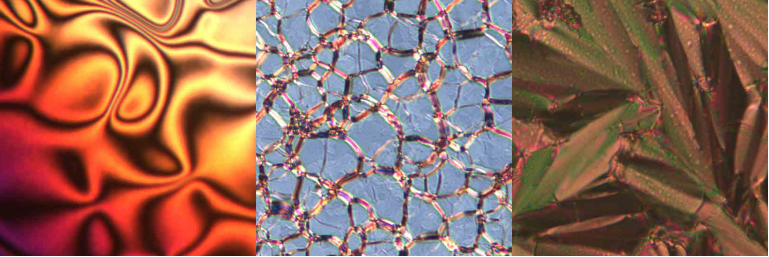
\includegraphics[width=6in]{images/texture_samples.png}
\caption{Liquid crystal textures from the dataset, from left to right: nematic phase compound 5CB, cholesteric phase compound D5, and smectic C phase compound M10.}
\end{figure}
%=========================================================================================
\section{General machine learning principles}
A machine learning model is a computer algorithm which automatically improves its performance in a given task as it gains experience from a dataset \cite{Goodfellow16}. It learns patterns in data and uses these patterns to make probabilistic predictions. The data normally takes the form of a set of $N$ examples, which are usually expressed as vectors, or some other structure of features, $\{\bm{x}^{(i)}\}_{i=1}^N$, containing quantitative information about example $i$. In supervised learning the examples are given labels $y^{(i)}$, to form a training set of pairs $\{\bm{x}^{(i)}, y^{(i)}\}_{i=1}^N$, and the model attempts to learn the mapping from a general input $\bm{x}$ to an output $\hat{y}$. One main type of supervised learning is regression, in which the output is a numerical scalar. The other main type is classification, in which the model predicts what the input belongs to out of a selection of classes. In unsupervised learning there are no labels, and the algorithm attempts to learn specific patterns in the dataset such as clusters of similar data points \cite{Murphy12}. The topic of this project is a supervised classification problem.

A supervised model can be usually be expressed as a function of inputs and a set of parameters $\boldsymbol\theta$ such that $\hat{y}=f(\bm{x};\boldsymbol\theta)$. Training involves optimisation of the parameters by minimisation of a cost function $J(\boldsymbol\theta)$, which measures the deviation of the predictions of the model from the true labels. The most common optimisation algorithms involve computing the gradient of $J(\boldsymbol\theta)$ with respect to $\boldsymbol\theta$ \cite{Goodfellow16}. 

The capacity of a model is akin to its complexity. The number of trainable parameters can give a fast indication of capacity. However, it also depends on the model's functional form. The parameters controlling the capacity of the model, as well as certain other training settings, are known as hyperparameters. If the capacity is too small, the model will tend to "underfit" the training set, resulting in poor performance even when optimised well. On the other hand, too high a capacity will result in "overfitting", with high performance on the training set, but the model may have a high generalisation error, which is the model's error rate when evaluating it on new, unseen data. Before training begins, the entire dataset is often split into training, validation, and test sets, containing $N_{\mathrm{train}}$, $N_{\mathrm{valid}}$ and $N_{\mathrm{test}}$ examples respectively. The training set, as defined previously, is used to optimise the parameters. The model's performance is then evaluated on the validation set. A poor performance on both the training and validation sets is indicative of underfitting, whereas a high performance on the training set and low on the validation set suggests overfitting. The validation set can therefore be used to tune the hyperparameters of the model before retraining. This can be repeated until the model fits optimally. The final model is then evaluated on the as-of-yet unseen test set to provide an estimate of its generalisation error. Methods used to reduce generalisation error, such as reducing model capacity, are known as regularisation. \cite{Goodfellow16}.
%=========================================================================================
\section{Feedforward neural networks}
A neural network is a type of machine learning model that takes inspiration from the current understanding of how the brain works. The inputs are "fed forward" through a series of connected "hidden units", akin to neurons in a brain, before reaching the output units. In the most basic form, a fully connected neural network, The units are arranged into layers, with each unit in a layer connected to every unit of the previous layer. We will define the total number of layers, excluding the input layer, as the depth, $D$, of the model, with the width, $W_l$, of layer $l\in[0..D]$ equal to the number of units it contains. $l=0$ is the input layer. The choice of the hyperparameters $D$ and $W_l$ defines the architecture of the model. A schematic of an example network is presented in Figure 2. 

\begin{figure}[h]
\centering
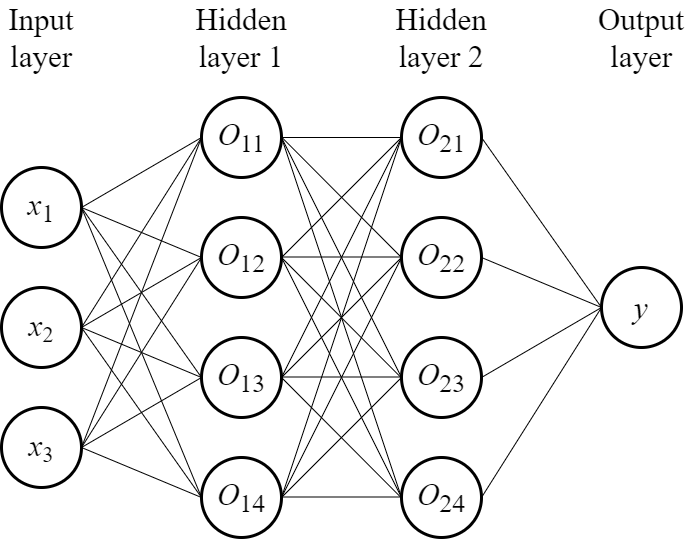
\includegraphics[width=3.5in]{images/feedforward_nn.png}
\caption{Diagram of a feedforward fully-connected neural network with three input values, $D=3$, $W_1=W_2=4$ and one output unit.}
\end{figure}

A single hidden unit's output value is calculated by multiplying the output of each of the previous layer's units with a weight parameter, summing these together with a bias parameter, and then passing the result through a non-linear activation function. More formally, the output $O_{lu}$ of hidden unit $u\in[1..W_l]$, of layer $l$, with bias parameter $b_{lu}$ and activation function $A(h)$ is calculated as
\begin{equation}
O_{lu}=A(h_{lu})
\end{equation}
with
\begin{equation}
h_{lu}=b_{lu}+\sum_{v=1}^{W_{l-1}}\theta_{luv}O_{(l-1)v}
\end{equation}
for $l > 0$. $\theta_{luv}$ is the weight parameter that hidden unit $u$ of layer $l$ applies to the output of unit $v\in[1..W_{l-1}]$ of the previous layer. $O_{0u}$, is equivalent to value $x_u$ of the the input vector $\bm{x}$. In matrix form,
\begin{equation}
\bm{O}_l=A(\bm{h}_l)
\end{equation}
with
\begin{equation}
\bm{h}_l=\boldsymbol\theta_l\bm{O}_{l-1}+\bm{b}_l
\end{equation}
where $\boldsymbol\theta_l$ is the $W_l \times \left(W_{l-1}\right)$ dimensional matrix of weights for layer $l$, with rows corresponding to the weights of each hidden unit, $\bm{O}_l$ is the vector of outputs for layer $l$, and $\bm{b}_l$ is the vector of bias parameters for layer $l$. The activation function is applied element-wise. For the first layer,
\begin{equation}
\bm{h}_1=\boldsymbol\theta_1\bm{x}+\bm{b_1}.
\end{equation}

The number of units in the final output layer depends on the type of model. For regression, there will be one unit that outputs a continuous-valued prediction. For classification, the number of final layer units is equal to the number of classes, $C=W_D$, with each one outputting the predicted probability that an input $\bm{x}$ belongs to a particular class. The network is therefore summarised as $\hat{\bm{y}}=f(\bm{x};\boldsymbol\theta)$, with $\hat{\bm{y}}$ being the $C$ dimensional vector of output probabilities. Each example in the dataset is labelled by a vector $\bm{y}$ with a value of one for the component corresponding to the true class, and zero for all other components. The component $y_u$, with $u\in[1..C]$, is equivalent to the Kronecker delta $\delta_{ut}$ where the index $t$ corresponds to the true class. The most common choice of final layer activation function for classification is the softmax function, $\sigma_{SM}(h)$, in which case the components $\hat{y}_u$ of the output probability prediction vector, are given by
\begin{equation}
\hat{y}_u=O_{Du}=\frac{e^{h_{Du}}}{\sum_{v=1}^{C}e^{h_{Dv}}}.
\end{equation} 
When there are just two classes, known as binary classification, only one unit is needed in the output layer. The data labels $y$ are equal to one or zero depending on the class that $\bm{x}$ belongs to. The activation function in this case is generally the logistic sigmoid function, $\sigma(h)$, with
\begin{equation}
\hat{y}=O_D=\frac{1}{1+e^{-h_D}}
\end{equation}
where in this situation $\boldsymbol\theta_D$ is a $W_{D-1}$ dimensional vector. The value of $\hat{y}$ is the predicted probability that $\bm{x}$ belongs to one of the classes, with a probability of $1-\hat{y}$ that it belongs to the other. The current most commonly used activation function for hidden units is the rectified linear unit (ReLU),
\begin{equation}
A(h)=\mathrm{max}(0,h).
\end{equation}
In 1989 Kurt Hornik \textit{et al.} mathematically proved that feedforward neural networks with multiple layers and non-linear activations can approximate any continuous function given the correct configuration \cite{Hornik89}. Another advantage of neural networks is that they can automatically learn to extract useful higher-level features from the raw input data.

\subsection{Neural network training}
Neural network training starts with random initialisation of the weights, for example by drawing values from a normal distribution. A single update step is generally carried out by calculating the model output for each example, followed by the gradient of the cost function with respect to the model weight parameters, $\bm{g}=\bm\nabla_{\bm\theta}J(\bm\theta)$. An iterative optimisation algorithm then uses the gradient to update the parameters to reduce the cost. $\bm{g}$ is obtained using the backpropagation algorithm, which calculates the gradient of $J(\bm\theta)$ with respect to the final outputs, and then recursively applies the chain rule going backwards through the network, calculating the derivatives with respect to the outputs of each hidden unit followed by their parameters. This algorithm is detailed in Appendix I. The overall goal of training iterations is to reduce the generalisation error of the model. Generally, the cost function is the expectation value of the loss of all examples in the training set,
\begin{equation}
J(\boldsymbol\theta)=\frac{1}{N_{\mathrm{train}}}\sum_{i=1}^{N_{\mathrm{train}}}L(f(\bm{x}^{(i)};\boldsymbol\theta),\bm{y}^{(i)})
\end{equation}
where the loss is the cross-entropy between the model's output probabilities and the input's true class label,
\begin{equation}
L(f(\bm{x};\boldsymbol\theta),\bm{y})=L(\hat{\bm{y}},\bm{y})=-\sum_{u=1}^Cy_u\mathrm{log}(\hat{y}_u).
\end{equation}
When training a classifier model, the softmax activation function of the final layer can be included in the loss function, to give the categorical cross-entropy,
\begin{equation}
L_{CCE}(\hat{\bm{y}},\bm{y})=-\sum_{u=1}^Cy_u\mathrm{log}\,\sigma_{SM}(h_{Du})=-\mathrm{log}\left(\frac{e^{h_{Dt}}}{\sum_{j=1}^{C}e^{h_{Dj}}}\right)
\end{equation}
where we have used the fact that $y_u=\delta_{ut}$ for classification. For binary classification in which the logistic sigmoid activation function is used, the binary cross-entropy is
\begin{equation}
L_{BCE}(\hat{y},y)=
\left\{
\begin{array}{ll}
-\mathrm{log}\,\sigma(h_D)  & \mbox{if } y^{(\mathrm{true})}=1 \\
-\mathrm{log}\left(1-\sigma(h_D)\right) & \mbox{if } y^{(\mathrm{true})}=0
\end{array}
\right..
\end{equation}

Calculating the exact derivative of the cost function is extremely computationally expensive in most situations when $N_{\mathrm{train}}$ is large. Instead, an approximation of the gradient, $\hat{\bm{g}}$, is calculated by randomly sampling a small batch of $m$ examples from the training data, giving
\begin{equation}
\hat{\bm{g}}=\frac{1}{m}\bm\nabla_{\bm\theta}\sum_{i=1}^mL(f(\bm{x}^{(i)};\boldsymbol\theta),\bm{y}^{(i)}).
\end{equation}
In general the performance loss from the difference between $\hat{\bm{g}}$ and the exact gradient $\bm{g}$ is outweighed by the greatly decreased training step computation time. Optimisation methods that use this random batch sampling are known as stochastic methods. Typically parameter update steps are performed batch by batch, with no duplicate example selections, until the whole training set has been seen by the model. After this all examples are again available for selection. Such a cycle is known as an epoch of training, with $\mathrm{floor}(N_{\mathrm{train}}/m)$ update steps.

Stochastic gradient descent (SGD) is a basic batch-based optimisation algorithm in which the parameters are updated in the opposite direction of $\hat{\bm{g}}$,
\begin{equation}
\bm\theta\leftarrow\bm\theta-\epsilon\hat{\bm{g}}
\end{equation}
where $\epsilon$ is a hyperparameter called the learning rate, which controls the amount by which the parameters change with each update. $\epsilon$ must be chosen carefully because it greatly affects the training stability and duration. For large neural networks the cost function has a highly irregular multi-dimensional form with many local minima, meaning that in general the final model will not find the global minimum. However, a local minimum is often enough to achieve low generalisation error. For all models trained in this project, the Adam optimisation algorithm was used, detailed in Appendix II. This is a type of SGD in which the learning rate at each step is adjusted based on unbiased estimates of the first and second moments of the gradient. This algorithm is less prone to becoming stuck in shallow local minima and is not too sensitive to the choice of its hyperparameters. 

\subsection{Neural network regularisation}
Neural networks can be prone to overfitting, especially ones with a high capacity or where the dataset is small. Good regularisation is therefore a requirement for models to perform well on the test set. There are a variety of strategies, from which the key ones used in this project are dataset augmentation, early stopping, and dropout.

Augmentation involves adding extra examples to the training set that are altered versions of the originals, increasing the effective overall number of training examples and reducing the chance of overfitting. The same effect can also be achieved by performing specific random transformations on each example as they are selected for each training batch. For example, image data can undergo random rotations, reflections, translations, magnification and other transformations. Of course, this must produces images that could still feasibly be a member of the original dataset.

If a model is trained for too many epochs, the performance on the training set may still be improving, but the generalisation error will start to increase due to overfitting. Early stopping aims to prevent this. A model performance measure, typically the cost function evaluated on a random batch from the validation set, is monitored during training. If after a specified number of epochs the performance has not improved by more than a tolerance value, the training will be stopped. The number of epochs allowed for improvement is called the patience hyperparameter.

When using dropout, at each training step hidden units are randomly chosen to not be included in the step, by multiplying their output by zero. The probability for a unit with dropout to not be included is equal to the dropout rate hyperparameter, which is often set to $\frac{1}{2}$. When applied applied to certain individual layers or to all hidden units, dropout simulates the training of many sub-models that all share parameters, encouraging each hidden unit to learn more general and useful features. This improves regularisation by increasing the final model's robustness to noise \cite{Srivastava2014}.

%=========================================================================================
\section{Convolutional neural networks}
CNNs are neural networks in which at least one layer uses the convolution operation to propagate information from the previous layer, instead of the standard fully-connected configuration. They have proven to be extremely effective at processing inputs with a large number of grid-like features, in particular image data. CNNs are trained in the same way as standard fully connected neural networks.
\subsection{Convolutional layers}
For image-based CNNs, a convolutional layer takes an input tensor $\bm{I}$ with width $W_I$, height $H_I$ and depth $D_I$, where the depth is the number of channels. Grayscale images have one channel, with a value corresponding to the brightness of the pixel at that location, whereas colour images have three channels, corresponding to the red, green and blue values for the pixel. The input is convolved with $N_K$ kernels, which are tensors $\bm{K}^{(d)}$ with width $W_K<W_I$, height $H_K<H_I$ and depth $D_K=D_I$. This produces a pre-activation output tensor $\bm{\bm{h}}$, which in the most basic case has width $W_h=W_I$, height $H_h=H_I$ and depth $D_h=N_KD_I$. $\bm{I}$ is convolved with each $\bm{K}^{(l)}$ in turn, with each output stacked together depth-wise to give the total output $\bm{h}$. Having more than one kernel increases the number of channels in the next layer. This overall operation is given by
\begin{equation}
h_{ijk}=\sum_{m=1}^{H_K}\sum_{n=1}^{W_K}I_{(i-m)(j-n)r}K_{mnr}^{(d)}
\end{equation}
with $r=k\,\mathrm{mod}\,D_I$ and $d=\lceil\frac{k}{D_I}\rceil$. Similarly to standard fully connected, or dense, hidden layers, an activation function is applied to every element of $\bm{h}$. 

Using more than one kernel allows a convolutional layer to extract more features from its input, at the cost of increased computation time and memory usage. The trainable parameters are the elements of the kernels. The kernels can individually learn different features to extract from the input, with the size of the features being related to the height and width dimensions of the kernels. The usage of kernels in convolutional layers is a form of parameter sharing, which is when parameters are used for more than one operation in a model. Compared to a dense layer, many less parameters are needed, resulting in greatly reduced memory consumption, and often improved regularisation. 

At the edges of the input, we have to consider the type of padding to use. Valid padding is when the kernel is kept completely within the bounds of the input, which results in the output having a smaller width and height than the input depending on the kernel size. The case we have discussed in which the width and height of the output are equal to the input corresponds to same padding, where each pixel is visited by the kernel the same number of times, resulting in it overlapping the boundary of the input at the furthest points. Any kernel parameters outside the input region are multiplied by zero.

Another adjustable property of convolutional layers is the stride. This is the number of elements by which the kernel is moved with each step. The stride can be different for the horizontal and vertical directions. The basic case of Equation 15 corresponds to a stride of one in both directions. Strides greater than one result in dimensionality reduction from input to output, with less feature extraction. However, this reduces computational cost for the layer.

\subsection{Pooling layers}
Convolutional layers are often directly followed by pooling. A pooling layer takes rectangles of a specific size, called the pool size, from the output of the previous layer. It outputs single values as a function of the values in each rectangle, similarly to how kernels work in convolutional layers. However, the function used by a pooling layer does not contain any trainable parameters, and each channel is processed individually. Padding and stride are also defined for pooling layers, in the same way as for convolutional layers. As an example, a pooling layer with pool size and strides of $2 \times 2$, valid padding, and input with dimensions $10 \times 10 \times 3$ will produce an output with dimensions $5 \times 5 \times 3$. There are a variety of pooling functions, such as max pooling, where the outputs are the maximum values in each rectangle, and average pooling, where the outputs are the means of the rectangles. Global pooling layers are a special case with a pool size equal to the width and height of the input, resulting in one output value for each of the input channels. The output is therefore a vector, suitable to be fed into a dense layer.

Pooling layers are utilised for two key reasons. Firstly, they can reduce the dimensions of the network between convolutional layers, decreasing computational cost. Secondly, they can make the CNN partially invariant to translations of features in the input.
%=========================================================================================
\section{Model training configurations}
All CNN models in this project have been implemented using the TensorFlow machine learning library with Keras high-level API, and were trained using NVIDIA CUDA on an NVIDIA RTX 2060 graphics processing unit. For every model, a batch size of $m=32$, the Adam optimiser with hyperparameters $\epsilon=0.001$, $\beta_1=0.9$, $\beta_2=0.999$ and $\delta=10^{-7}$ and early stopping  monitored by validation set loss and with a patience of 100 epochs was used.
%=========================================================================================
\section{4-phase classifier models}

\subsection{Dataset preparation}

\subsection{Model architectures and training configuration}

\subsection{Results}

%=========================================================================================
\section{Smectic A and C binary classifier models}

\subsection{Dataset preparation}

\subsection{Model architectures and training configuration}

\subsection{Results}

%=========================================================================================
\section{General smectic phase classifier models}

\subsection{Dataset preparation}

\subsection{Model architectures and training configuration}

\subsection{Results}

%=========================================================================================
\section{Conclusions}

%=========================================================================================
\section{Going forward}

%=========================================================================================

\bibliography{report}

\appendix
\appendixpage
\section{Backpropagation}
\section{Adam optimiser}
Before the first iteration, the biased first and second moment estimate variables $\bm{s}$ and $\bm{r}$ are initialised to zero. At the start of an iteration, a batch of data is sampled and $\hat{\bm{g}}$ is calculated as in Equation 13. $\bm{s}$ is updated as
\begin{equation}
\bm{s}
\end{equation}        

\end{document}